\documentclass{article}
\usepackage{tikz}

\begin{document}

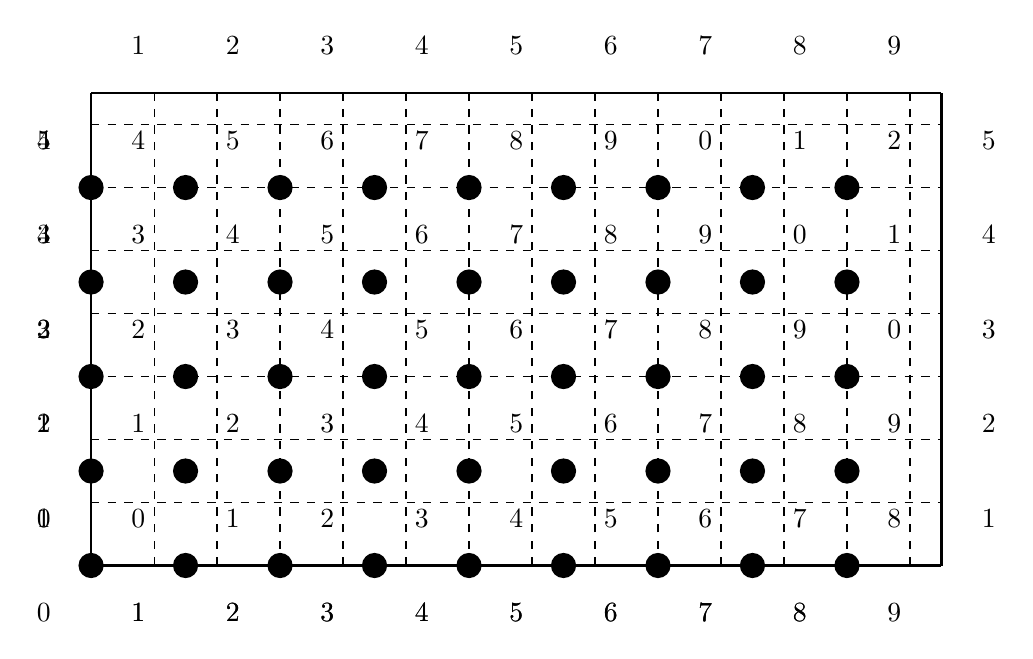
\begin{tikzpicture}[scale=0.8]
    \def\rowdist{1.5}
    \def\coldist{1.5}
    
    % Draw the grid lines
    \draw[dashed] (0,0) grid (9*\coldist, 5*\rowdist);
    
    % Label the rows
    \foreach \y [count=\i from 0] in {0,...,4} {
        \node at (-0.5*\coldist, \i*\rowdist + 0.5*\rowdist) {\i};
    }
    
    % Label the columns
    \foreach \x [count=\i from 0] in {0,...,8} {
        \node at (\i*\coldist - 0.5*\coldist, -0.5*\rowdist) {\i};
    }
    
    % Place the vertices
    \foreach \x in {0,...,8} {
        \foreach \y in {0,...,4} {
            \pgfmathtruncatemacro{\color}{mod(\x+\y, 10)}
            \ifnum\color=0
                \fill[red] (\x*\coldist, \y*\rowdist) circle (0.2);
            \else
                \ifnum\color=1
                    \fill[blue] (\x*\coldist, \y*\rowdist) circle (0.2);
                \else
                    \fill[black] (\x*\coldist, \y*\rowdist) circle (0.2);
                \fi
            \fi
        }
    }
    
    % Draw the edges
    \draw[thick] (0,0) -- (0,5*\rowdist);
    \draw[thick] (9*\coldist,0) -- (9*\coldist,5*\rowdist);
    \draw[thick] (0,0) -- (9*\coldist,0);
    \draw[thick] (0,5*\rowdist) -- (9*\coldist,5*\rowdist);
    
    % Add the labels inside the cells
    \foreach \x in {0,...,8} {
        \foreach \y in {0,...,4} {
            \pgfmathtruncatemacro{\label}{mod(\x+\y, 10)}
            \node at (\x*\coldist + 0.5*\coldist, \y*\rowdist + 0.5*\rowdist) {\label};
        }
    }
    
    % Draw the dashed lines between specific vertices
    \draw[dashed] (0,0) -- (9*\coldist,0);
    \draw[dashed] (0,5*\rowdist) -- (9*\coldist,5*\rowdist);
    \draw[dashed] (0,0) -- (0,5*\rowdist);
    \draw[dashed] (9*\coldist,0) -- (9*\coldist,5*\rowdist);
    
    % Add the labels for the dashed lines
    \foreach \x in {0,...,8} {
        \pgfmathtruncatemacro{\label}{mod(\x+1, 10)}
        \node at (\x*\coldist + 0.5*\coldist, -0.5*\rowdist) {\label};
    }
    
    % Add the labels for the dashed lines on the right side
    \foreach \y in {0,...,4} {
        \pgfmathtruncatemacro{\label}{mod(\y+1, 10)}
        \node at (9*\coldist + 0.5*\coldist, \y*\rowdist + 0.5*\rowdist) {\label};
    }
    
    % Add the labels for the dashed lines on the bottom
    \foreach \x in {0,...,8} {
        \pgfmathtruncatemacro{\label}{mod(\x+1, 10)}
        \node at (\x*\coldist + 0.5*\coldist, 5*\rowdist + 0.5*\rowdist) {\label};
    }
    
    % Add the labels for the dashed lines on the top
    \foreach \y in {0,...,4} {
        \pgfmathtruncatemacro{\label}{mod(\y+1, 10)}
        \node at (-0.5*\coldist, \y*\rowdist + 0.5*\rowdist) {\label};
    }
\end{tikzpicture}

\end{document}